
%(BEGIN_QUESTION)
% Copyright 2012, Tony R. Kuphaldt, released under the Creative Commons Attribution License (v 1.0)
% This means you may do almost anything with this work of mine, so long as you give me proper credit

Undersøk denne prosessen, der temperaturen i vannet nederst i en ``water seal drum''-beholder reguleres ved å føre varm damp gjennom et varmerør nedsenket i vannet:

$$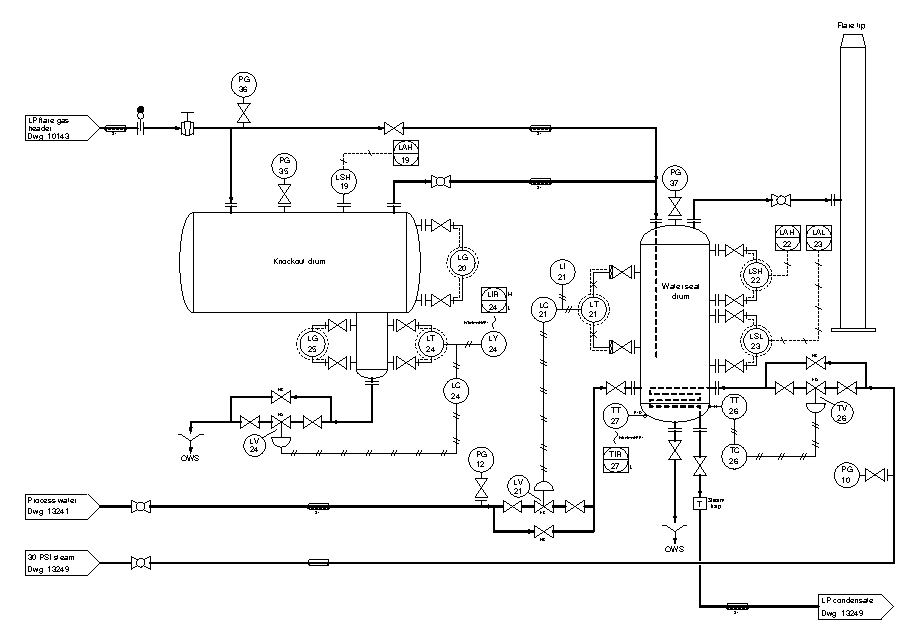
\includegraphics[width=15.5cm]{i0002rx01.eps}$$

Anta at dampkjelen for 30 PSI dampforsyning en dag stopper, slik at dampstrømmen til TV-26 opphører. Uten damp til oppvarming av seal drum begynner vannet å kjøles ned. Hva vil regulator TC-26 gjøre som respons på denne hendelsen, forutsatt at den er en regulator med proporsjonal + integralvirkning (P+I)?

Anta nå at dette dampavbruddet varer svært lenge. Hvordan vil regulatorens proporsjonal- og integralmodus reagere dersom regulatoren står i automatisk hele tiden? Finnes det en måte å unngå dette problemet på?
 
\vskip 20pt \vbox{\hrule \hbox{\strut \vrule{} {\bf Forslag til sokratisk diskusjon} \vrule} \hrule}

\begin{itemize}
\item{} Når du ser på diagrammet, hva tror du funksjonen til water seal drum er i den større sammenhengen i flare-prosessen?
\item{} Hva er verst tenkelig scenario: at vannet i seal drum blir for kaldt eller for varmt? Hvordan kan vi se det ut fra detaljene i diagrammet?
\item{} Anta at driftsorganisasjonen ber deg installere instrumentering for å måle total mengde stoff som slippes til fakkel hver måned, for utslippsoppfølging. For dem som har studert flowmålere: identifiser minst én praktisk løsning på dette, inkludert hvilke teknologier som kan brukes for å måle dampene som går til fakkel.
\end{itemize}

\underbar{file i01608}
%(END_QUESTION)





%(BEGIN_ANSWER)

Regulatoren vil redusere utgangssignalet sitt mens den forsøker å åpne air-to-close-ventilen. Både proporsjonal- og integralleddet i regulatoren vil arbeide for å åpne dampventilen når reaktortemperaturen synker. Hvis dampforsyningen er borte over lengre tid, vil regulatorens integralvirkning {\it vinde} til metning (3 PSI eller lavere utgangssignaltrykk).

%(END_ANSWER)





%(BEGIN_NOTES)

Vannet i seal drum vil naturligvis ikke varmes opp igjen før dampforsyningen er tilbake, uansett hvilken stilling regulatoren setter dampreguleringsventilen i.

Integral ``windup'' kan nullstilles ved å sette regulatoren i manuell modus og så tilbake til automatisk. Interne ``windup limits'' kan settes for å bidra til å hindre at dette skjer senere.

\vskip 10pt

Én løsning på det sokratiske spørsmålet om hvordan total flaret mengde kan måles, er å plassere en ultrasonisk flowmåler i fakkelledningen og deretter totalisere (integrere) flowmålingen. En annen løsning er å måle strålingsvarmeeffekten fra flammen og integrere den (for å beregne total brent BTU).









\filbreak \vskip 20pt \vbox{\hrule \hbox{\strut \vrule{} {\bf Virtuell feilsøking} \vrule} \hrule}

\noindent
{\bf Forutsi virkningen av en gitt feil:} presenter hver av følgende feil for studentene, én om gangen, og la dem kommentere alle virkningene hver feil vil gi.

\begin{itemize}
\item{} 
\item{} 
\item{} 
\end{itemize}


\vskip 10pt


\noindent
{\bf Identifisere mulige/umulige feil:} presenter symptomer for studentene, og la dem deretter avgjøre om en serie foreslåtte feil kan forklare alle symptomene, med begrunnelse for {\it hvorfor} eller {\it hvorfor ikke} for hver foreslåtte feil:

\begin{itemize}
\item{} Symptom: {\it }
\item{} 
\item{} 
\item{} 
\end{itemize}


\vskip 10pt


\noindent
{\bf Bestemme nytten av diagnostiske tester:} presenter symptomer for studentene, og foreslå deretter følgende diagnostiske tester én etter én. Studentene vurderer nytten av hver test, altså om den gir nyttig informasjon (forteller oss noe vi ikke allerede vet). Studentene vurderer også hva ulike testresultater eventuelt vil indikere om feilen:

\begin{itemize}
\item{} Symptom: {\it }
\item{}  -- {\bf Ja/Nei}
\item{}  -- {\bf Ja/Nei}
\end{itemize}


\vskip 10pt


\noindent
{\bf Diagnostisere en feil ut fra gitte symptomer:} tenk deg at dysen tetter seg i LC-21, slik at nivåreguleringsventilen åpner fullt og flommer water seal drum med vann (ikke avslør feilen for studentene!). Presenter operatørens observasjon(er), la studentene vurdere mulige feil og teststrategier, og gi dem deretter resultatene av testene de foreslår basert på symptomene under, helt til de har identifisert feiltype og feilplassering korrekt:

\begin{itemize}
\item{} {\it Operatørene mottar en høy-nivå alarm LAH-22}
\item{} LT-21 mottaker-måler viser 16 PSI
\item{} LV-21 står helt åpen
\item{} TC-26 er under setpunkt (PV = 50 deg F ; SP = 100 deg F)
\item{} PG-36 og PG-37 viser begge oscillerende trykkavlesninger (periodiske støt)
\item{} {\it Første tiltak når problemet er identifisert?}
\end{itemize}


%INDEX% Control, integral: windup
%INDEX% Process: steam-heated reactor vessel (generic)

%(END_NOTES)
